\section{Trigonometri}
\subsection{Basics}
\begin{figure}
    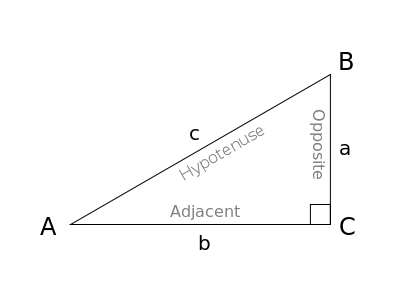
\includegraphics[width=0.8\textwidth]{trig_basic}
\end{figure}

\begin{math}
	\sin A=\frac{\textrm{opposite}}{\textrm{hypotenuse}}=\frac{a}{\,c\,}\,.
\end{math} \\[2pt]
\begin{math}
	\cos A=\frac{\textrm{adjacent}}{\textrm{hypotenuse}}=\frac{b}{\,c\,}\,.
\end{math} \\[2pt]

\subsection{Kraftuppdelning}

\begin{figure}
    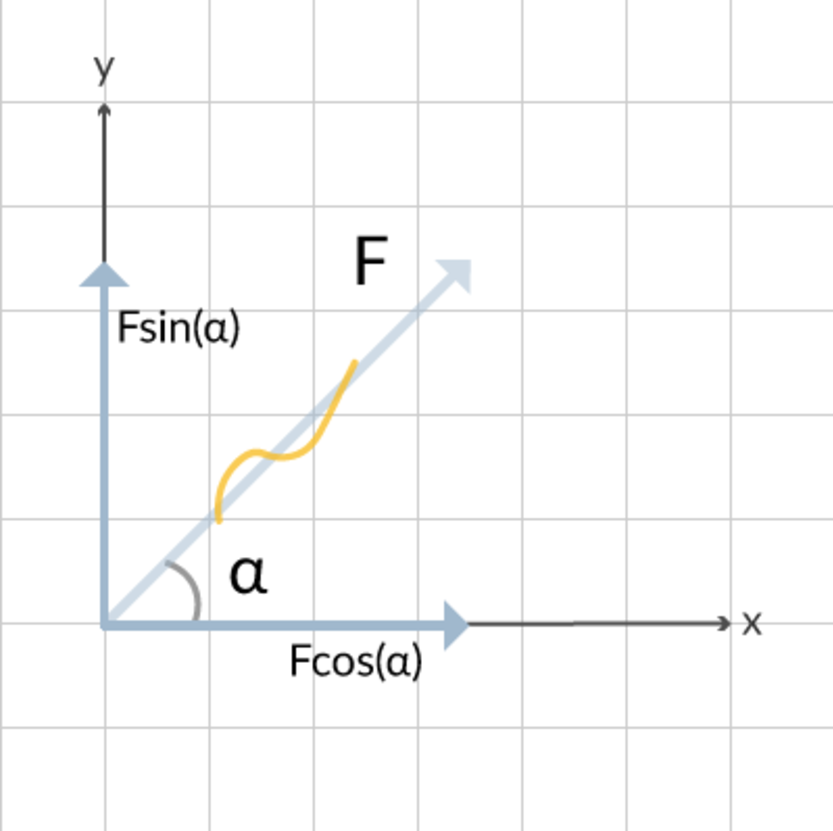
\includegraphics[width=0.8\textwidth]{uppdelning}
\end{figure}
